\documentclass[]{beamer}
%\documentclass{article}
%\usepackage{beamerarticle}


\mode<presentation>
{
  \usetheme{Warsaw}
  % or ...

  \setbeamercovered{transparent}
  % or whatever (possibly just delete it)
}


\usepackage[english]{babel}
% or whatever

\usepackage[utf8]{inputenc}
% or whatever

\usepackage{times}
\usepackage[T1]{fontenc}
\usepackage{tikz}
\usetikzlibrary{arrows.meta}

%%%%%%%%%%%%%%%%%%%%%%%%%%%%%%%%%%
%%                         PACKAGES                      %%
%%%%%%%%%%%%%%%%%%%%%%%%%%%%%%%%%%
\usepackage{hyperref,ctable}
\usepackage{graphicx}
\usepackage{tikz}                    % For flowchart
\usetikzlibrary{shapes,arrows} % For flowchart
\usetikzlibrary{arrows.meta}



%%%%%%%%%%%%%%%%%%%%%%%%%%%%%%%%%%
%%                           COLORS                        %%
%%%%%%%%%%%%%%%%%%%%%%%%%%%%%%%%%%
%AU COLORS
\definecolor{aublue}{RGB}{25,33,129}
\definecolor{aured}{RGB}{244,28,31}

%Red
%\setbeamercolor{titlelike}{bg=aured,fg=white}
\setbeamercolor{structure}{bg=black!25!aured, fg=aured}
%\setbeamercolor*{palette primary}{fg=white,bg=aured}
%\setbeamercolor*{palette quaternary}{fg=white,bg=aublue}

%Blue
\setbeamercolor{titlelike}{bg=aublue,fg=white}
%\setbeamercolor{structure}{bg=black!25!aublue, fg=aublue}
\setbeamercolor*{palette primary}{fg=white,bg=aublue}
\setbeamercolor*{palette quaternary}{fg=white,bg=black!75!aublue}

\setbeamercolor{local structure}{fg=aured,bg=gray!60!aured}
\setbeamercolor{alerted text}{fg=aured}

\newenvironment{concept}[1]%
	{
	\setbeamercolor{background canvas}{bg=aured!10!white}%
	\setbeamercolor{frametitle}{bg=aured}%
	\setbeamercolor{frametitle right}{bg=aured}
	\setbeamercolor{alerted text}{fg=aured}%
	\begin{frame}{Concept}%
	\alert{\bfseries \large #1\\[2em]}}{%
	\end{frame}%
	}


%%%%%%%%%%%%%%%%%%%%%%%%%%%%%%%%%%
%%                         GRAPHICS                       %%
%%%%%%%%%%%%%%%%%%%%%%%%%%%%%%%%%%
%\graphicspath{{/Users/bader/work/Presentations/Images/}}}}


%%%%%%%%%%%%%%%%%%%%%%%%%%%%%%%%%%
%%                        COMMANDS                       %%
%%%%%%%%%%%%%%%%%%%%%%%%%%%%%%%%%%
\newcommand{\strong}[1]{\textbf{#1}}
\AtBeginSection[]{
  \begin{frame}
  \vfill
  \centering
  \begin{beamercolorbox}[sep=8pt,center,shadow=true,rounded=true]{title}
    \usebeamerfont{title}\insertsectionhead\par%
  \end{beamercolorbox}
  \vfill
  \end{frame}
}
\AtBeginSubsection{\frame{\subsectionpage}}



%%%%%%%%%%%%%%%%%%%%%%%%%%%%%%%%%%
%%                     PRESENTATION                   %%
%%%%%%%%%%%%%%%%%%%%%%%%%%%%%%%%%%
\title[Review]{Semester Review}

\author[Bader--SOCY 625]
{Michael D.~M.~Bader}

\institute 
{
  Practicum in Sociological Research (SOCY 625)
}
% - Use the \inst command only if there are several affiliations.
% - Keep it simple, no one is interested in your street address.

\date % (optional)
{Week 14}

\subject{Practicum in Sociological Research Slides}
% This is only inserted into the PDF information catalog. Can be left
% out.

% If you have a file called "university-logo-filename.xxx", where xxx
% is a graphic format that can be processed by latex or pdflatex,
% resp., then you can add a logo as follows:

%\logo{\includegraphics[height=1cm]{../../Images/au_logo_50by51px}}
%\logo{\includegraphics[height=1cm]{../../Images/au_logoname_300}}
\logo{\includegraphics[height=1cm]{/Users/bader/work/Presentations/Images/au_logoname_300}}

\subject{Intro to Survey Methods}
% This is only inserted into the PDF information catalog. Can be left
% out. 



% If you have a file called "university-logo-filename.xxx", where xxx
% is a graphic format that can be processed by latex or pdflatex,
% resp., then you can add a logo as follows:

% \pgfdeclareimage[height=0.5cm]{university-logo}{university-logo-filename}
% \logo{\pgfuseimage{university-logo}}



% Delete this, if you do not want the table of contents to pop up at
% the beginning of each subsection:
%\AtBeginSubsection[]
%{
%  \begin{frame}<beamer>{Outline}
%    \tableofcontents[currentsection,currentsubsection]
%  \end{frame}
%}


% If you wish to uncover everything in a step-wise fashion, uncomment
% the following command: 

%\beamerdefaultoverlayspecification{<+->}


\begin{document}

\begin{frame}
  \titlepage
\end{frame}

\section{Questions about the Workshop?}

\section{Review}

\begin{frame}
\textbf{Major Concepts:}
\begin{itemize}
\item Inference \pause
\item Error \pause
	\begin{itemize}
	\item Validity \pause
	\item Reliability \pause
	\item Bias \pause
	\end{itemize}
\item Variance 
\end{itemize}
\end{frame}

\begin{frame}
\begin{center}
\includegraphics[scale=.75]{../../Week2-InferenceAndError/images/GrovesCh2Fig2.pdf}
\end{center}
\end{frame}

\subsection{Measurement}

\begin{frame}
\begin{center}
\includegraphics[scale=.75]{../../Week2-InferenceAndError/images/GrovesCh2Fig2Measurement.pdf}
\end{center}
\end{frame}

\begin{concept}{construct}{elements of information sought by the researcher (Groves, et al., 41)}
\end{concept}

\begin{concept}{measurement}{how we ask our questions to measure our construct of interest}
\end{concept}

\begin{concept}{response}{how a respondent understands, interprets, and responds to our measurement (questions)}
\end{concept}

\begin{frame}
\begin{center}
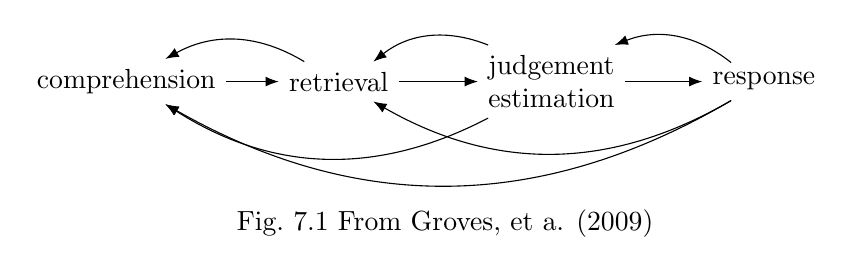
\begin{tikzpicture}[scale=.9]
\usetikzlibrary{arrows.meta}

\node [align=center, thick] (comp)  at (0,0) {comprehension};
\node [align=center, thick] (retr) at (3,0) {retrieval};
\node [align=center, thick] (judg) at (6,0) {judgement\\estimation};
\node [align=center, thick] (resp) at (9,0) {response};

\path [-Latex] (comp) edge (retr) (retr) edge (judg) (judg) edge (resp);
\draw [-Latex] (resp) to [bend right] (judg);
\draw [-Latex] (judg) to [bend right] (retr);
\draw [-Latex] (retr) to [bend right] (comp);
\draw [-Latex] (resp) to [bend left] (retr);
\draw [-Latex] (judg) to [bend left] (comp);
\draw [-Latex] (resp) to [bend left] (comp);

\node [align=center] at (4.5,-2) {Fig.\ 7.1 From Groves, et a. (2009)};

\end{tikzpicture}
\end{center}
\end{frame}

\begin{concept}{edited response}{the response ultimately used in our analysis}\end{concept}

\begin{concept}{edited response}{the response ultimately used in our analysis}\end{concept}

\subsection{Representation}

\begin{frame}
\begin{center}
\includegraphics[scale=.75]{../../Week2-InferenceAndError/images/GrovesCh2Fig2Representation.pdf}
\end{center}
\end{frame}


\begin{concept}{target population}{group of elements (people) that we want to represent with our survey}\end{concept}

\begin{concept}{sampling frame}{the enumerated list of elements in the target population from which we will draw our sample}\end{concept}

\begin{concept}{sample}{a subset of elements drawn from the sampling frame; in survey research, that should be based on a \emph{probabilistic sample}}\end{concept}

\begin{frame}
\begin{itemize}
\item All elements in the target population a non-zero probability of inclusion into the sample
\item All elements in the sampling frame have a known probability of inclusion into the sample
\item The elements of the sample are \emph{unbiased} with respect to the target population
\end{itemize}
\end{frame}

\begin{concept}{sampling variation}{the amount of variation around a population value due to random chances of drawing different samples from a population}
\end{concept}

\begin{frame}
Sampling variation (sampling error) will be \textbf{lower}:
\begin{enumerate}
\item with larger samples (though nonlinear)
\item with less variation in the measure
\end{enumerate} 
\end{frame}

\begin{frame}
\begin{center}
\includegraphics[width=4in]{../images/sampleSizePlot.jpeg}
\end{center}
\end{frame}

\begin{concept}{respondents}{people who actually answer questions on our instrument}
\end{concept}

\begin{frame}
\textbf{Non-response} (remember potential for bias):
\begin{itemize}
\item Unit non-response
\item Item non-response
\end{itemize}
\end{frame}

\begin{concept}{survey weights}{factor by which each respondent should be multiplied to have the sample represent known quantities in the target population\\[1em](in simple cases equal to the inverse of the probability of inclusion in the sample)}
\end{concept}

\begin{frame}
\begin{description}
\item[Clustered sample] Sample primary sampling units (PSUs) and then sample from within those PSUs (tends to increase design effect)
\item[Stratified sample] Sample from different strata of the population to ensure representation (tends to decrease design effect)
\end{description}
\end{frame}


\begin{frame}
\begin{center}
\includegraphics[scale=.75]{../../Week2-InferenceAndError/images/GrovesCh2Fig2.pdf}
\end{center}
\end{frame}

\end{document}


